\documentclass{presentation}

\title{Συναρτήσεις}
\subtitle{Πράξεις Συναρτήσεων}
\author[Λόλας]{Κωνσταντίνος Λόλας }
\institute[$10^ο$ ΓΕΛ]{$10^ο$ ΓΕΛ Θεσσαλονίκης}
\date{}

\begin{document}

\begin{frame}
  \titlepage
\end{frame}
\begin{frame}{Ισότητα Συναρτήσεων}
  \begin{block}{Ορισμός}
    Δύο συναρτήσεις $f$ και $g$ θα είναι ίσες αν:
    \begin{itemize}
      \item έχουν ίδιο πεδίο ορισμού $Α$
      \item $f(x)=g(x)$ για κάθε $x\in Α$
    \end{itemize}
  \end{block}
\end{frame}

\begin{frame}{Πράξεις Συναρτήσεων}
  \begin{block}{Πρόσθεση}
    Έστω $f(x)$, $x\in Α$ και $g(x)$, $x\in Β$ δύο συναρτήσεις. Η συνάρτηση $(f+g)(x)$ έχει
    \begin{itemize}
      \item Πεδίο ορισμού το $A\cap Β$
      \item Κανόνα $f(x)+g(x)$
    \end{itemize}
  \end{block}
\end{frame}

\begin{frame}{Πράξεις Συναρτήσεων}
  \begin{block}{Πράξεις}
    Έστω $f(x)$, $x\in Α$ και $g(x)$, $x\in Β$ δύο συναρτήσεις.
    \begin{itemize}
      \item $(f-g)(x)=f(x)-g(x)$, $x\in A\cap Β$
      \item $(f\cdot g)(x)=f(x)\cdot g(x)$, $x\in A\cap Β$
      \item $(f/g)(x)=f(x)/g(x)$, $x\in A\cap Β$ και $g(x)\ne 0$
    \end{itemize}
  \end{block}
\end{frame}

\begin{frame}{Και κάτι καινούριο}
  \begin{block}{Σύνθεση της $g$ με την $f$}
    Έστω $f(x)$, $x\in Α$ και $g(x)$, $x\in Β$ δύο συναρτήσεις. Η συνάρτηση $(f\circ g)(x)$ έχει
    \begin{itemize}
      \item Κανόνα $f(g(x))$
      \item Πεδίο ορισμού το $\{x\in Β | g(x)\in Α \}$
    \end{itemize}
  \end{block}
  \centering
  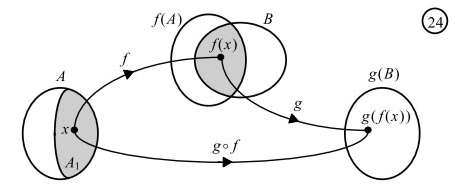
\includegraphics[width=0.5\textwidth]{"images/1.2 Σύνθεση.png"}
\end{frame}

\begin{frame}{Δύσκολο; Μπα}
  \begin{block}{Σύνθεση}
    Έστω $f(x)$, $x\in Α$ και $g(x)$, $x\in Β$ δύο συναρτήσεις. Η συνάρτηση $(f\circ g)(x)$ έχει
    \begin{itemize}
      \item Κανόνα $f(g(x))$
      \item Ορίζεται αν $Α\cap g(Β)\ne \emptyset$
            \begin{itemize}
              \item<2-> $x\in Β$
              \item<3-> $g(x)\in Α$
              \item<4-> τύπος είναι απλά αντικατάσταση
            \end{itemize}
    \end{itemize}
  \end{block}
\end{frame}

\section{Ασκήσεις}

\begin{askisi}
  Να εξετάσετε αν οι συναρτήσεις:
  $$f(x)=x-\ln (e^x-1) \text{ και } g(x)=\ln\frac{e^x}{e^x-1}$$
  είναι ίσες

  %\hyperlink{Λύση1}{\beamerbutton{Λύση}}
\end{askisi}

\begin{askisi}
  Δίνονται οι συναρτήσεις $f(x)=x^{\frac{2}{3}}$ και $g(x)=\sqrt[3]{x^2}$
  \begin{enumerate}
    \item<1-> Να εξετάσετε αν οι συναρτήσεις είναι ίσες
    \item<2-> Αν $f\ne g$ να βρείτε το ευρύτερο υποσύνολο του $\mathbb{R}$ στο οποίο να ισχύει $f=g$
    \item<3-> Να γράψετε τη συνάρτηση $g$ σε μορφή δύναμης
  \end{enumerate}

  %\hyperlink{Λύση2}{\beamerbutton{Λύση}}
\end{askisi}

\begin{askisi}
  Δίνονται οι συναρτήσεις $f(x)=\sqrt{e^x-1}$ και $g(x)=\frac{x-1}{x-2}$
  Να βρείτε τις συναρτήσεις:
  \begin{enumerate}
    \item<1-> $f+g$
    \item<2-> $\frac{1}{g}$
    \item<3-> $\frac{f}{g}$
  \end{enumerate}

  %\hyperlink{Λύση3}{\beamerbutton{Λύση}}
\end{askisi}

\begin{askisi}
  Να βρείτε τη συνάρτηση $f$ για την οποία ισχύει
  $$f^2(x)=4e^x\left(f(x)-e^x\right)$$

  %\hyperlink{Λύση4}{\beamerbutton{Λύση}}
\end{askisi}

\begin{askisi}
  Δίνονται οι συναρτήσεις $f(x)=\sqrt{x-1}$ και $g(x)=\frac{1}{x}$. Να βρείτε τις συναρτήσεις
  \begin{enumerate}
    \item<1-> $f\circ g$
    \item<2-> $g\circ f$
    \item<3-> $f\circ f$
  \end{enumerate}

  %\hyperlink{Λύση5}{\beamerbutton{Λύση}}
\end{askisi}

\begin{askisi}
  Δίνονται οι συναρτήσεις $f(x)=\frac{x+1}{x-1}$ και $g(x)=\frac{1}{x}$. Να βρείτε τις συναρτήσειςs
  \begin{enumerate}
    \item<1-> $f\circ g$
    \item<2-> $g\circ \frac{1}{f}$
  \end{enumerate}

  %\hyperlink{Λύση6}{\beamerbutton{Λύση}}
\end{askisi}

\begin{askisi}
  Έστω $f:\mathbb{R}\to\mathbb{R}$ μία συνάρτηση, για την οποία ισχύει
  $$f(\ln x)=3x+2\ln x -1\text{, για κάθε } x>0$$
  Να βρείτε τη συνάρτηση $f$

  %\hyperlink{Λύση7}{\beamerbutton{Λύση}}
\end{askisi}

\begin{askisi}
  Έστω δύο συναρτήσεις για τις οποίες ισχύει
  $$(g\circ f)(x)=e^x-x+1\text{, } x\in\mathbb{R}$$
  \begin{enumerate}
    \item<1-> Να βρείτε τη συνάρτηση $g$, αν $f(x)=e^x-1$
    \item<2-> Να βρείτε τη συνάρτηση $f$, αν $g(x)=3x-2$
  \end{enumerate}

  %\hyperlink{Λύση8}{\beamerbutton{Λύση}}
\end{askisi}

\begin{askisi}
  Να εκφράσετε την συνάρτηση $f$ ώς σύνθεση δύο ή περισσοτέρων συναρτήσεων, αν ισχύει:
  \begin{itemize}
    \item $f(x)=ημ 3x$
    \item $f(x)=e^{-x}$
    \item $f(x)=\ln (1+e^x)$
  \end{itemize}

  %\hyperlink{Λύση9}{\beamerbutton{Λύση}}
\end{askisi}

\begin{askisi}
  Έστω $f:\mathbb{R}\to\mathbb{R}$ μία συνάρτηση, για την οποία ισχύει:
  $$f^3(x)+f(x)-x+2=0\text{, για κάθε } x\in\mathbb{R}$$
  \begin{enumerate}
    \item<1-> Να βρείτε το $f(0)$
    \item<2-> Να βρείτε τις ρίζες και το πρόσημο της $f$
    \item<3-> Να λύσετε την ανίσωση $f(x)<x-2$
    \item<4-> Αν θεωρήσουμε γνωστό ότι το σύνολο της $f$ είναι το $\mathbb{R}$, να δείξετε ότι η εξίσωση $e^{f(x)}-2023=0$ έχει μία τουλάχιστον λύση
  \end{enumerate}

  %\hyperlink{Λύση10}{\beamerbutton{Λύση}}
\end{askisi}

\begin{askisi}
  Έστω $f:\mathbb{R}\to\mathbb{R}$ μία συνάρτηση, για την οποία ισχύει:
  $$f(x^2+2)+f(3x)=0 \text{, για κάθε } x\in\mathbb{R}$$
  Να δείξετε ότι η εξίσωση $f(x)=0$ έχει δύο τουλάχιστον ρίζες.

  %\hyperlink{Λύση11}{\beamerbutton{Λύση}}
\end{askisi}

\begin{askisi}
  Έστω $f:\mathbb{R}\to\mathbb{R}$ μία συνάρτηση, για την οποία ισχύει:
  $$f\left(f(x)\right)=2x-1\text{, για κάθε } x\in\mathbb{R}$$
  \begin{enumerate}
    \item<1-> Να δείξετε ότι $f(2x-1)=2f(x)-1$, $x\in\mathbb{R}$
    \item<2-> Να δείξετε ότι η εξίσωση $f(x)=1$ έχει μία τουλάχιστον ρίζα
  \end{enumerate}

  %\hyperlink{Λύση12}{\beamerbutton{Λύση}}
\end{askisi}

\end{document}
